\documentclass[12pt]{article}
\usepackage[table]{xcolor}
\usepackage[shortlabels]{enumitem}
\usepackage{tabularx,xltabular}
\usepackage{graphicx}
\usepackage{hyperref}
\usepackage{verbatim}
\usepackage{geometry}
\usepackage{ulem}
\usepackage[official]{eurosym}
\usepackage{tikz}
\usetikzlibrary{arrows,backgrounds,calc,decorations.markings,patterns,3d}
\usepackage{pgfplots}
\pgfplotsset{compat = newest}
\usetikzlibrary{fit}
\newcommand\addvmargin[1]{
\usetikzlibrary{arrows}
\node[fit=(current bounding box),inner ysep=#1,inner xsep=0]{};}
\usepackage{cancel}
\usepackage{fontspec}
\usepackage{array}  
\geometry{a4paper, top=2cm, left=2cm, right=2cm, bottom=2cm, headsep=1cm}
\usepackage{tabu}
\usepackage{pst-node}
\usepackage{colortbl}
\usepackage{array}
\usepackage{german}
\setlength\parindent{0pt}
\newcolumntype{?}{!{\vrule width 1pt}}
\usepackage{makecell}
\renewcommand{\arraystretch}{2.5}
\usepackage{pbox}
\usepackage{amssymb}
\usepackage{amsmath}
\usepackage{booktabs}
\newcolumntype{L}[1]{>{\raggedright\let\newline\\\arraybackslash\hspace{0pt}}m{#1}}
\newcolumntype{C}[1]{>{\centering\let\newline\\\arraybackslash\hspace{0pt}}m{#1}}
\newcolumntype{R}[1]{>{\raggedleft\let\newline\\\arraybackslash\hspace{0pt}}m{#1}}
\begin{document}
\rightline{Datum: 08.06.2023}
\centerline{{\Large Tägliche Übungen}} 
\vspace{1cm}
\noindent \\


\begin{xltabular}{\textwidth}{|C{0.75cm}|X|C{0.75cm}|X|}
\arrayrulecolor{black}\hline
a)&$\begin{aligned}
 x=&-9~ \rightarrow ~ 2 \cdot x - 2 \cdot x=?
\end{aligned}$
&
b)&$\begin{aligned}
 b=&2~ \rightarrow ~ 5 \cdot b - 3=?
\end{aligned}$
\\\hline
c)&$\begin{aligned}
 z=&-5~ \rightarrow ~ z + 3=?
\end{aligned}$
&
d)&$\begin{aligned}
 a=&-1~ \rightarrow ~ 4 \cdot a + 1=?
\end{aligned}$
\\\hline
e)&$3\cdot y-13=14$
&
f)&$4\cdot b-18=30$
\\\hline
g)&$2\cdot b-6=14$
&
h)&$7\cdot x-15=41$
\\\hline
i)&$10\cdot x-12=28$
&
j)&$5\cdot y-5=5$
\\\hline
k)&$9\cdot y-13=41$
&
l)&$7\cdot a-8=76$
\\\hline
m)&$6\cdot a-3=51$
&
n)&$8\cdot y-16=32$
\\\hline
o)&$6\cdot b-14=4$
&
p)&$4\cdot b-4=20$
\\\hline
q)&$6\cdot y-20=52$
&
r)&$8\cdot a-13=83$
\\\hline
s)&$10\cdot y-15=75$
&
t)&$5\cdot b-7=48$
\\\hline
u)&$3\cdot a-18=-3$
&
v)&$4\cdot b-6=14$
\\\hline
w)&$10\cdot y-12=88$
&
x)&$6\cdot a-3=69$
\\\hline
y)&$7\cdot x-6=36$
&
z)&$4\cdot y-17=31$
\\\hline
\end{xltabular}
\vspace{0.5cm}
\newpage
\rightline{Datum: 08.06.2023}
\centerline{{\large Lösungen Tägliche Übungen}} 
\vspace{0.5cm}

\begin{xltabular}{\textwidth}{|C{0.75cm}|X|C{0.75cm}|X|}
\arrayrulecolor{black}\hline
a)&$\begin{aligned}
\textcolor{red}{x=-9} & \rightarrow\\
2 \cdot x - 2 \cdot x=&2 \cdot \textcolor{red}{(-9)} - 2 \cdot \textcolor{red}{(-9)}=0\\
\end{aligned}$
&
b)&$\begin{aligned}
\textcolor{red}{b=2} & \rightarrow\\
5 \cdot b - 3=&5 \cdot \textcolor{red}{2} - 3=7\\
\end{aligned}$
\\\hline
c)&$\begin{aligned}
\textcolor{red}{z=-5} & \rightarrow\\
z + 3=&\textcolor{red}{(-5)} + 3=-2\\
\end{aligned}$
&
d)&$\begin{aligned}
\textcolor{red}{a=-1} & \rightarrow\\
4 \cdot a + 1=&4 \cdot \textcolor{red}{(-1)} + 1=-3\\
\end{aligned}$
\\\hline
e)&\begingroup\setlength{\jot}{-0.03cm}
\tikzstyle{background grid}=[draw, black!15,step=.5cm]
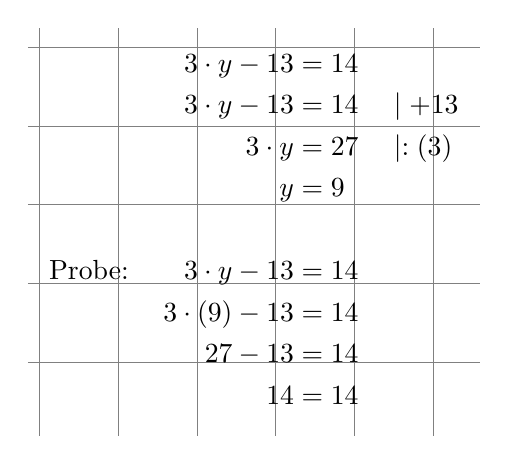
\begin{tikzpicture}[show background grid]
\node[below right] at (0,0.1) {
$\begin{aligned}
3\cdot y-13 &=14& &  \\
3\cdot y - 13 &=14& & \mid + 13\\
3\cdot y &=27& & \mid :\left(3\right)\\
y &=9& & 
\\
\\
\mbox{Probe:}\qquad 3\cdot y-13 &=14& &  \\
3\cdot \left(9\right)-13 &=14& &  \\
27-13 &=14& &  \\
14 &=14& &  \\
\end{aligned}$};
\end{tikzpicture}
\endgroup
&
f)&\begingroup\setlength{\jot}{-0.03cm}
\tikzstyle{background grid}=[draw, black!15,step=.5cm]
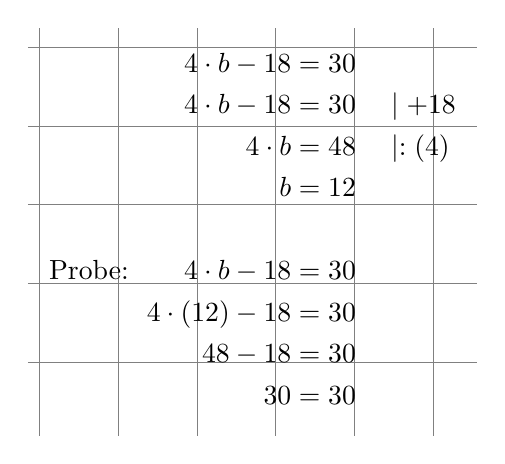
\begin{tikzpicture}[show background grid]
\node[below right] at (0,0.1) {
$\begin{aligned}
4\cdot b-18 &=30& &  \\
4\cdot b - 18 &=30& & \mid + 18\\
4\cdot b &=48& & \mid :\left(4\right)\\
b &=12& & 
\\
\\
\mbox{Probe:}\qquad 4\cdot b-18 &=30& &  \\
4\cdot \left(12\right)-18 &=30& &  \\
48-18 &=30& &  \\
30 &=30& &  \\
\end{aligned}$};
\end{tikzpicture}
\endgroup
\\\hline
g)&\begingroup\setlength{\jot}{-0.03cm}
\tikzstyle{background grid}=[draw, black!15,step=.5cm]
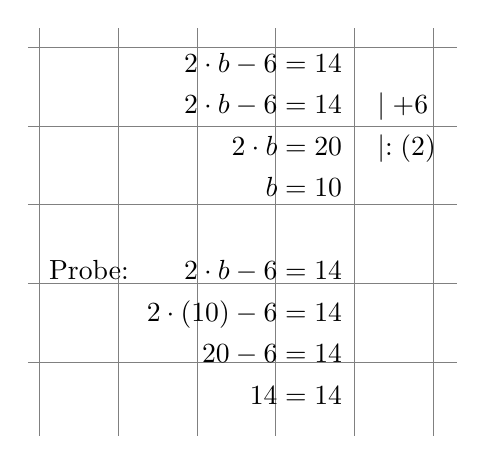
\begin{tikzpicture}[show background grid]
\node[below right] at (0,0.1) {
$\begin{aligned}
2\cdot b-6 &=14& &  \\
2\cdot b - 6 &=14& & \mid + 6\\
2\cdot b &=20& & \mid :\left(2\right)\\
b &=10& & 
\\
\\
\mbox{Probe:}\qquad 2\cdot b-6 &=14& &  \\
2\cdot \left(10\right)-6 &=14& &  \\
20-6 &=14& &  \\
14 &=14& &  \\
\end{aligned}$};
\end{tikzpicture}
\endgroup
&
h)&\begingroup\setlength{\jot}{-0.03cm}
\tikzstyle{background grid}=[draw, black!15,step=.5cm]
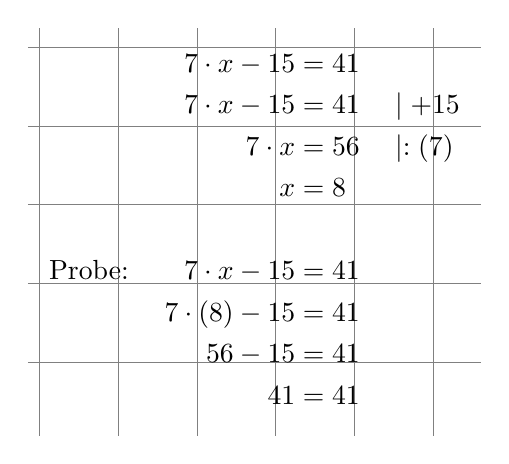
\begin{tikzpicture}[show background grid]
\node[below right] at (0,0.1) {
$\begin{aligned}
7\cdot x-15 &=41& &  \\
7\cdot x - 15 &=41& & \mid + 15\\
7\cdot x &=56& & \mid :\left(7\right)\\
x &=8& & 
\\
\\
\mbox{Probe:}\qquad 7\cdot x-15 &=41& &  \\
7\cdot \left(8\right)-15 &=41& &  \\
56-15 &=41& &  \\
41 &=41& &  \\
\end{aligned}$};
\end{tikzpicture}
\endgroup
\\\hline
i)&\begingroup\setlength{\jot}{-0.03cm}
\tikzstyle{background grid}=[draw, black!15,step=.5cm]
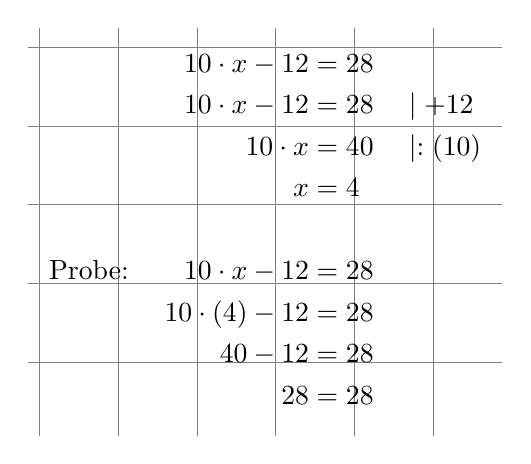
\begin{tikzpicture}[show background grid]
\node[below right] at (0,0.1) {
$\begin{aligned}
10\cdot x-12 &=28& &  \\
10\cdot x - 12 &=28& & \mid + 12\\
10\cdot x &=40& & \mid :\left(10\right)\\
x &=4& & 
\\
\\
\mbox{Probe:}\qquad 10\cdot x-12 &=28& &  \\
10\cdot \left(4\right)-12 &=28& &  \\
40-12 &=28& &  \\
28 &=28& &  \\
\end{aligned}$};
\end{tikzpicture}
\endgroup
&
j)&\begingroup\setlength{\jot}{-0.03cm}
\tikzstyle{background grid}=[draw, black!15,step=.5cm]
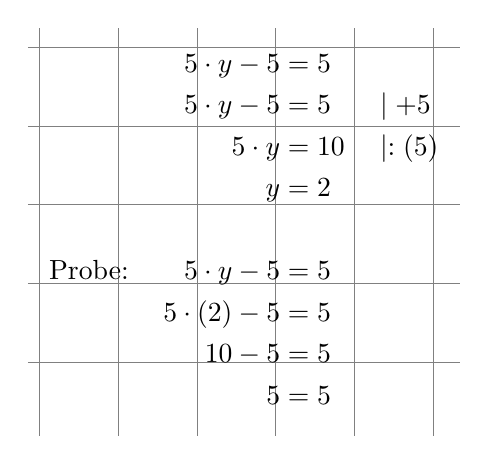
\begin{tikzpicture}[show background grid]
\node[below right] at (0,0.1) {
$\begin{aligned}
5\cdot y-5 &=5& &  \\
5\cdot y - 5 &=5& & \mid + 5\\
5\cdot y &=10& & \mid :\left(5\right)\\
y &=2& & 
\\
\\
\mbox{Probe:}\qquad 5\cdot y-5 &=5& &  \\
5\cdot \left(2\right)-5 &=5& &  \\
10-5 &=5& &  \\
5 &=5& &  \\
\end{aligned}$};
\end{tikzpicture}
\endgroup
\\\hline
k)&\begingroup\setlength{\jot}{-0.03cm}
\tikzstyle{background grid}=[draw, black!15,step=.5cm]
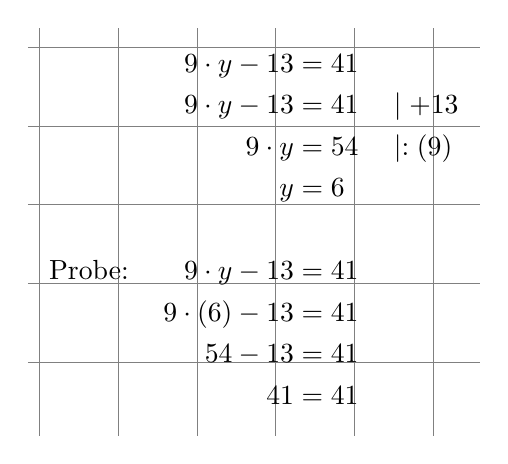
\begin{tikzpicture}[show background grid]
\node[below right] at (0,0.1) {
$\begin{aligned}
9\cdot y-13 &=41& &  \\
9\cdot y - 13 &=41& & \mid + 13\\
9\cdot y &=54& & \mid :\left(9\right)\\
y &=6& & 
\\
\\
\mbox{Probe:}\qquad 9\cdot y-13 &=41& &  \\
9\cdot \left(6\right)-13 &=41& &  \\
54-13 &=41& &  \\
41 &=41& &  \\
\end{aligned}$};
\end{tikzpicture}
\endgroup
&
l)&\begingroup\setlength{\jot}{-0.03cm}
\tikzstyle{background grid}=[draw, black!15,step=.5cm]
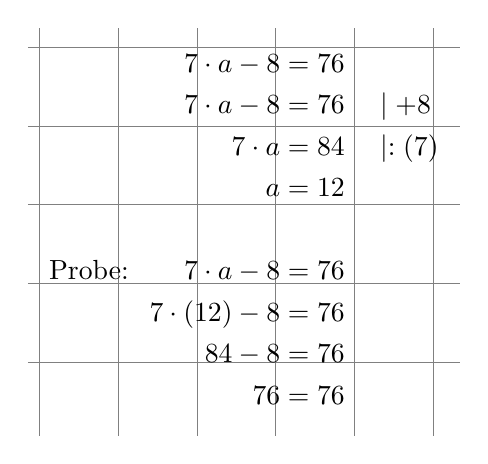
\begin{tikzpicture}[show background grid]
\node[below right] at (0,0.1) {
$\begin{aligned}
7\cdot a-8 &=76& &  \\
7\cdot a - 8 &=76& & \mid + 8\\
7\cdot a &=84& & \mid :\left(7\right)\\
a &=12& & 
\\
\\
\mbox{Probe:}\qquad 7\cdot a-8 &=76& &  \\
7\cdot \left(12\right)-8 &=76& &  \\
84-8 &=76& &  \\
76 &=76& &  \\
\end{aligned}$};
\end{tikzpicture}
\endgroup
\\\hline
m)&\begingroup\setlength{\jot}{-0.03cm}
\tikzstyle{background grid}=[draw, black!15,step=.5cm]
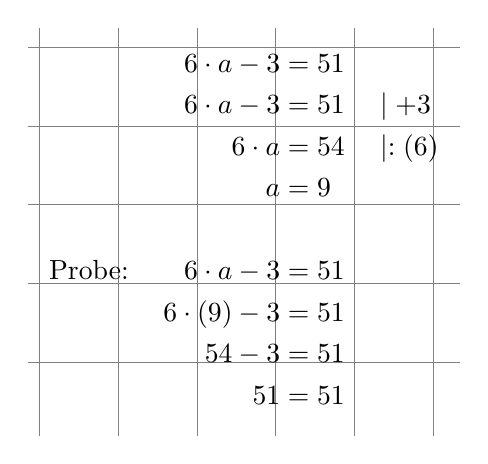
\begin{tikzpicture}[show background grid]
\node[below right] at (0,0.1) {
$\begin{aligned}
6\cdot a-3 &=51& &  \\
6\cdot a - 3 &=51& & \mid + 3\\
6\cdot a &=54& & \mid :\left(6\right)\\
a &=9& & 
\\
\\
\mbox{Probe:}\qquad 6\cdot a-3 &=51& &  \\
6\cdot \left(9\right)-3 &=51& &  \\
54-3 &=51& &  \\
51 &=51& &  \\
\end{aligned}$};
\end{tikzpicture}
\endgroup
&
n)&\begingroup\setlength{\jot}{-0.03cm}
\tikzstyle{background grid}=[draw, black!15,step=.5cm]
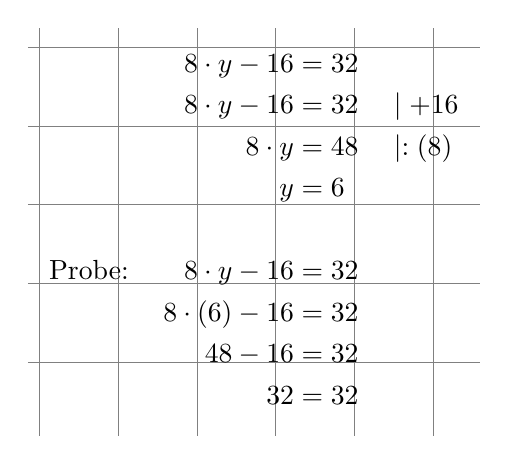
\begin{tikzpicture}[show background grid]
\node[below right] at (0,0.1) {
$\begin{aligned}
8\cdot y-16 &=32& &  \\
8\cdot y - 16 &=32& & \mid + 16\\
8\cdot y &=48& & \mid :\left(8\right)\\
y &=6& & 
\\
\\
\mbox{Probe:}\qquad 8\cdot y-16 &=32& &  \\
8\cdot \left(6\right)-16 &=32& &  \\
48-16 &=32& &  \\
32 &=32& &  \\
\end{aligned}$};
\end{tikzpicture}
\endgroup
\\\hline
o)&\begingroup\setlength{\jot}{-0.03cm}
\tikzstyle{background grid}=[draw, black!15,step=.5cm]
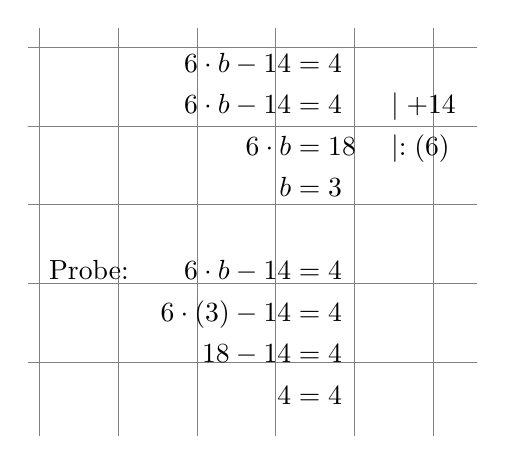
\begin{tikzpicture}[show background grid]
\node[below right] at (0,0.1) {
$\begin{aligned}
6\cdot b-14 &=4& &  \\
6\cdot b - 14 &=4& & \mid + 14\\
6\cdot b &=18& & \mid :\left(6\right)\\
b &=3& & 
\\
\\
\mbox{Probe:}\qquad 6\cdot b-14 &=4& &  \\
6\cdot \left(3\right)-14 &=4& &  \\
18-14 &=4& &  \\
4 &=4& &  \\
\end{aligned}$};
\end{tikzpicture}
\endgroup
&
p)&\begingroup\setlength{\jot}{-0.03cm}
\tikzstyle{background grid}=[draw, black!15,step=.5cm]
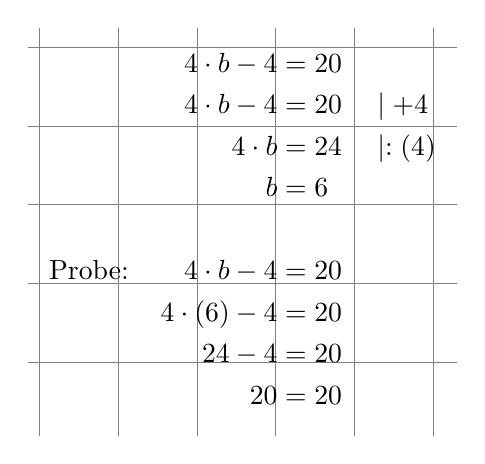
\begin{tikzpicture}[show background grid]
\node[below right] at (0,0.1) {
$\begin{aligned}
4\cdot b-4 &=20& &  \\
4\cdot b - 4 &=20& & \mid + 4\\
4\cdot b &=24& & \mid :\left(4\right)\\
b &=6& & 
\\
\\
\mbox{Probe:}\qquad 4\cdot b-4 &=20& &  \\
4\cdot \left(6\right)-4 &=20& &  \\
24-4 &=20& &  \\
20 &=20& &  \\
\end{aligned}$};
\end{tikzpicture}
\endgroup
\\\hline
q)&\begingroup\setlength{\jot}{-0.03cm}
\tikzstyle{background grid}=[draw, black!15,step=.5cm]
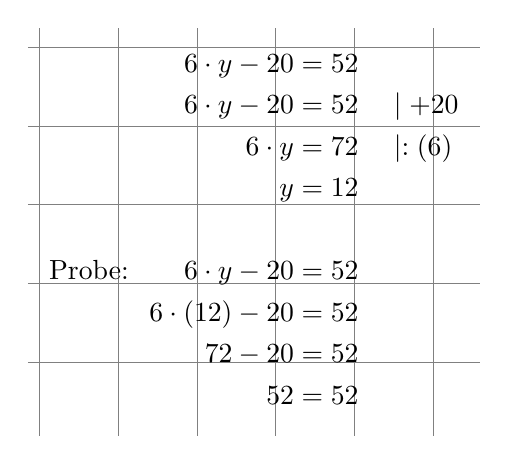
\begin{tikzpicture}[show background grid]
\node[below right] at (0,0.1) {
$\begin{aligned}
6\cdot y-20 &=52& &  \\
6\cdot y - 20 &=52& & \mid + 20\\
6\cdot y &=72& & \mid :\left(6\right)\\
y &=12& & 
\\
\\
\mbox{Probe:}\qquad 6\cdot y-20 &=52& &  \\
6\cdot \left(12\right)-20 &=52& &  \\
72-20 &=52& &  \\
52 &=52& &  \\
\end{aligned}$};
\end{tikzpicture}
\endgroup
&
r)&\begingroup\setlength{\jot}{-0.03cm}
\tikzstyle{background grid}=[draw, black!15,step=.5cm]
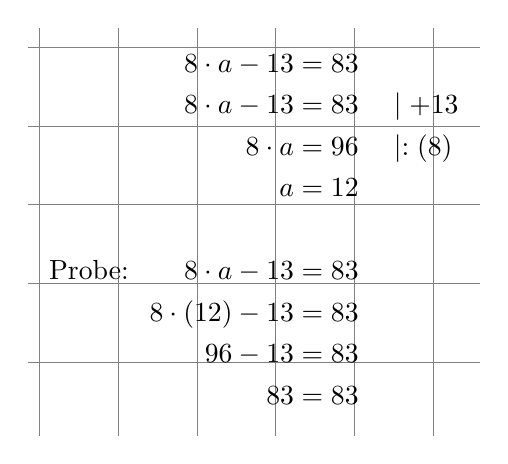
\begin{tikzpicture}[show background grid]
\node[below right] at (0,0.1) {
$\begin{aligned}
8\cdot a-13 &=83& &  \\
8\cdot a - 13 &=83& & \mid + 13\\
8\cdot a &=96& & \mid :\left(8\right)\\
a &=12& & 
\\
\\
\mbox{Probe:}\qquad 8\cdot a-13 &=83& &  \\
8\cdot \left(12\right)-13 &=83& &  \\
96-13 &=83& &  \\
83 &=83& &  \\
\end{aligned}$};
\end{tikzpicture}
\endgroup
\\\hline
s)&\begingroup\setlength{\jot}{-0.03cm}
\tikzstyle{background grid}=[draw, black!15,step=.5cm]
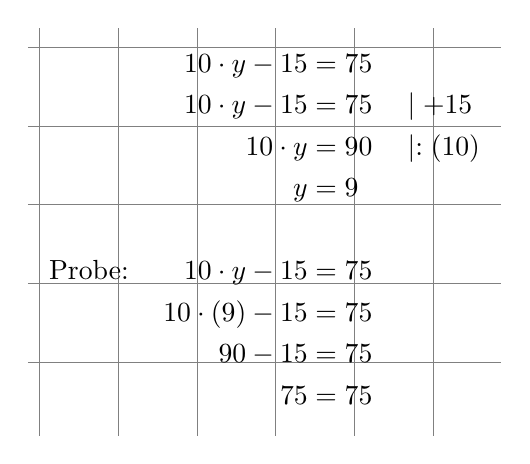
\begin{tikzpicture}[show background grid]
\node[below right] at (0,0.1) {
$\begin{aligned}
10\cdot y-15 &=75& &  \\
10\cdot y - 15 &=75& & \mid + 15\\
10\cdot y &=90& & \mid :\left(10\right)\\
y &=9& & 
\\
\\
\mbox{Probe:}\qquad 10\cdot y-15 &=75& &  \\
10\cdot \left(9\right)-15 &=75& &  \\
90-15 &=75& &  \\
75 &=75& &  \\
\end{aligned}$};
\end{tikzpicture}
\endgroup
&
t)&\begingroup\setlength{\jot}{-0.03cm}
\tikzstyle{background grid}=[draw, black!15,step=.5cm]
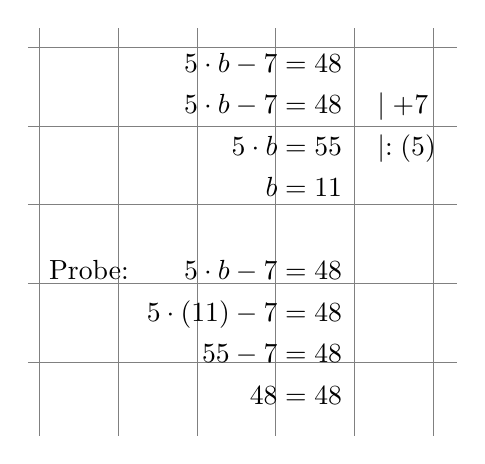
\begin{tikzpicture}[show background grid]
\node[below right] at (0,0.1) {
$\begin{aligned}
5\cdot b-7 &=48& &  \\
5\cdot b - 7 &=48& & \mid + 7\\
5\cdot b &=55& & \mid :\left(5\right)\\
b &=11& & 
\\
\\
\mbox{Probe:}\qquad 5\cdot b-7 &=48& &  \\
5\cdot \left(11\right)-7 &=48& &  \\
55-7 &=48& &  \\
48 &=48& &  \\
\end{aligned}$};
\end{tikzpicture}
\endgroup
\\\hline
u)&\begingroup\setlength{\jot}{-0.03cm}
\tikzstyle{background grid}=[draw, black!15,step=.5cm]
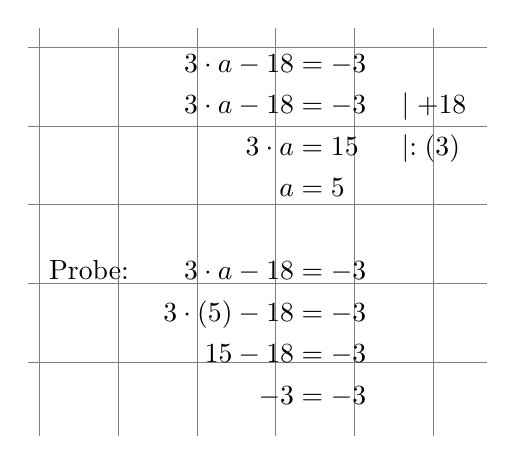
\begin{tikzpicture}[show background grid]
\node[below right] at (0,0.1) {
$\begin{aligned}
3\cdot a-18 &=-3& &  \\
3\cdot a - 18 &=-3& & \mid + 18\\
3\cdot a &=15& & \mid :\left(3\right)\\
a &=5& & 
\\
\\
\mbox{Probe:}\qquad 3\cdot a-18 &=-3& &  \\
3\cdot \left(5\right)-18 &=-3& &  \\
15-18 &=-3& &  \\
-3 &=-3& &  \\
\end{aligned}$};
\end{tikzpicture}
\endgroup
&
v)&\begingroup\setlength{\jot}{-0.03cm}
\tikzstyle{background grid}=[draw, black!15,step=.5cm]
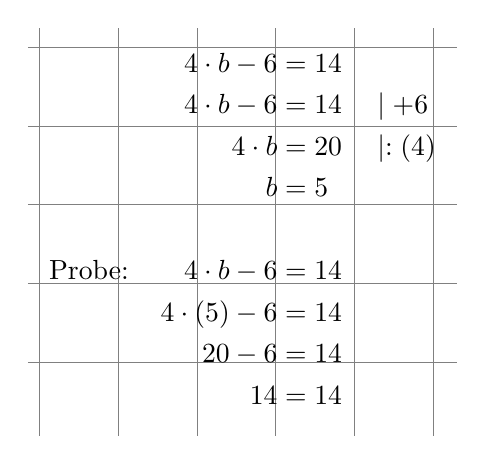
\begin{tikzpicture}[show background grid]
\node[below right] at (0,0.1) {
$\begin{aligned}
4\cdot b-6 &=14& &  \\
4\cdot b - 6 &=14& & \mid + 6\\
4\cdot b &=20& & \mid :\left(4\right)\\
b &=5& & 
\\
\\
\mbox{Probe:}\qquad 4\cdot b-6 &=14& &  \\
4\cdot \left(5\right)-6 &=14& &  \\
20-6 &=14& &  \\
14 &=14& &  \\
\end{aligned}$};
\end{tikzpicture}
\endgroup
\\\hline
w)&\begingroup\setlength{\jot}{-0.03cm}
\tikzstyle{background grid}=[draw, black!15,step=.5cm]
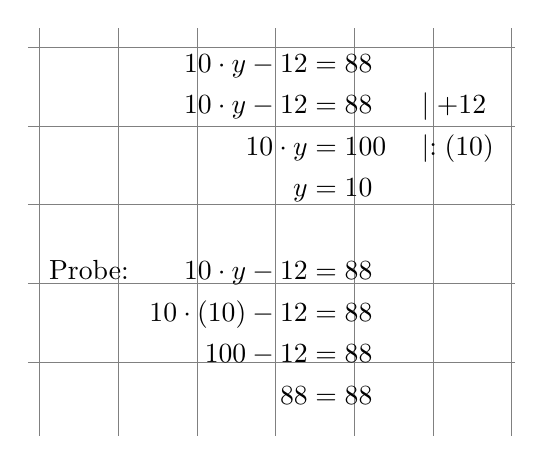
\begin{tikzpicture}[show background grid]
\node[below right] at (0,0.1) {
$\begin{aligned}
10\cdot y-12 &=88& &  \\
10\cdot y - 12 &=88& & \mid + 12\\
10\cdot y &=100& & \mid :\left(10\right)\\
y &=10& & 
\\
\\
\mbox{Probe:}\qquad 10\cdot y-12 &=88& &  \\
10\cdot \left(10\right)-12 &=88& &  \\
100-12 &=88& &  \\
88 &=88& &  \\
\end{aligned}$};
\end{tikzpicture}
\endgroup
&
x)&\begingroup\setlength{\jot}{-0.03cm}
\tikzstyle{background grid}=[draw, black!15,step=.5cm]
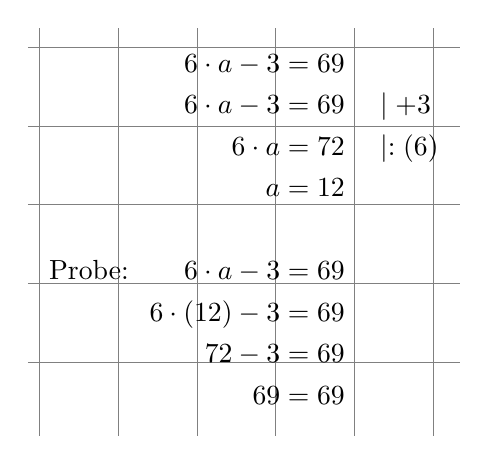
\begin{tikzpicture}[show background grid]
\node[below right] at (0,0.1) {
$\begin{aligned}
6\cdot a-3 &=69& &  \\
6\cdot a - 3 &=69& & \mid + 3\\
6\cdot a &=72& & \mid :\left(6\right)\\
a &=12& & 
\\
\\
\mbox{Probe:}\qquad 6\cdot a-3 &=69& &  \\
6\cdot \left(12\right)-3 &=69& &  \\
72-3 &=69& &  \\
69 &=69& &  \\
\end{aligned}$};
\end{tikzpicture}
\endgroup
\\\hline
y)&\begingroup\setlength{\jot}{-0.03cm}
\tikzstyle{background grid}=[draw, black!15,step=.5cm]
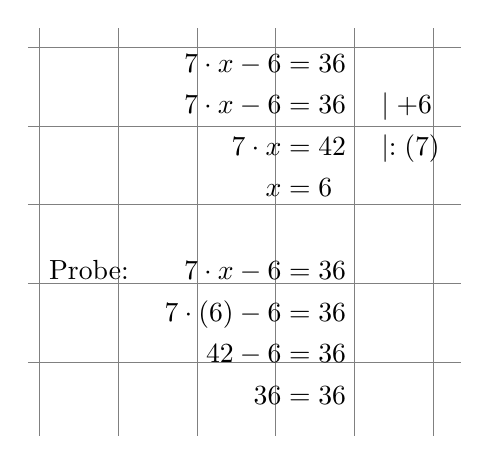
\begin{tikzpicture}[show background grid]
\node[below right] at (0,0.1) {
$\begin{aligned}
7\cdot x-6 &=36& &  \\
7\cdot x - 6 &=36& & \mid + 6\\
7\cdot x &=42& & \mid :\left(7\right)\\
x &=6& & 
\\
\\
\mbox{Probe:}\qquad 7\cdot x-6 &=36& &  \\
7\cdot \left(6\right)-6 &=36& &  \\
42-6 &=36& &  \\
36 &=36& &  \\
\end{aligned}$};
\end{tikzpicture}
\endgroup
&
z)&\begingroup\setlength{\jot}{-0.03cm}
\tikzstyle{background grid}=[draw, black!15,step=.5cm]
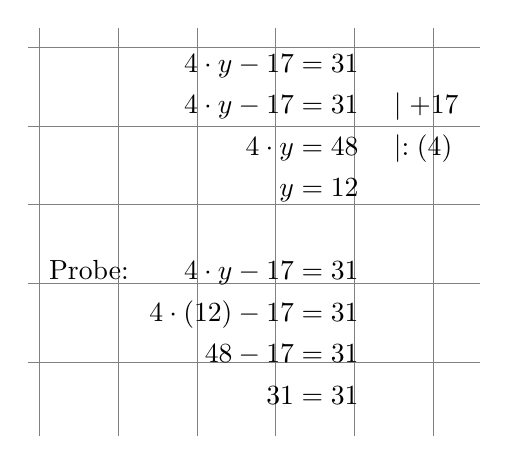
\begin{tikzpicture}[show background grid]
\node[below right] at (0,0.1) {
$\begin{aligned}
4\cdot y-17 &=31& &  \\
4\cdot y - 17 &=31& & \mid + 17\\
4\cdot y &=48& & \mid :\left(4\right)\\
y &=12& & 
\\
\\
\mbox{Probe:}\qquad 4\cdot y-17 &=31& &  \\
4\cdot \left(12\right)-17 &=31& &  \\
48-17 &=31& &  \\
31 &=31& &  \\
\end{aligned}$};
\end{tikzpicture}
\endgroup
\\\hline
\end{xltabular}
\vspace{0.5cm}
\end{document}